\chapter{Tree algorithms}

\index{tree}

A \key{tree} is a connected, acyclic graph
that consists of $n$ nodes and $n-1$ edges.
Removing any edge from a tree divides it
into two components,
and adding any edge to a tree creates a cycle.
Moreover, there is always a unique path between any
two nodes of a tree.

For example, the following tree consists of 8 nodes and 7 edges:
\begin{center}
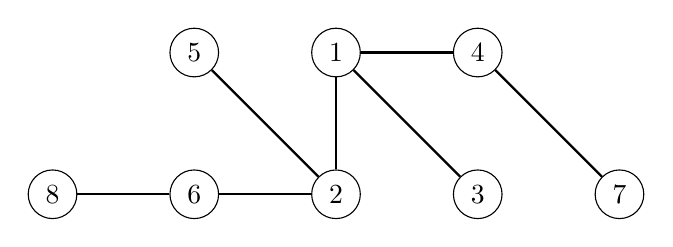
\begin{tikzpicture}[scale=0.9]
\node[draw, circle] (1) at (0,3) {$1$};
\node[draw, circle] (2) at (2,3) {$4$};
\node[draw, circle] (3) at (0,1) {$2$};
\node[draw, circle] (4) at (2,1) {$3$};
\node[draw, circle] (5) at (4,1) {$7$};
\node[draw, circle] (6) at (-2,3) {$5$};
\node[draw, circle] (7) at (-2,1) {$6$};
\node[draw, circle] (8) at (-4,1) {$8$};
\path[draw,thick,-] (1) -- (2);
\path[draw,thick,-] (1) -- (3);
\path[draw,thick,-] (1) -- (4);
\path[draw,thick,-] (2) -- (5);
\path[draw,thick,-] (3) -- (6);
\path[draw,thick,-] (3) -- (7);
\path[draw,thick,-] (7) -- (8);
\end{tikzpicture}
\end{center}

\index{leaf}

The \key{leaves} of a tree are the nodes
with degree 1, i.e., with only one neighbor.
For example, the leaves of the above tree
are nodes 3, 5, 7 and 8.

\index{root}
\index{rooted tree}

In a \key{rooted} tree, one of the nodes
is appointed the \key{root} of the tree,
and all other nodes are
placed underneath the root.
For example, in the following tree,
node 1 is the root node.

\begin{center}
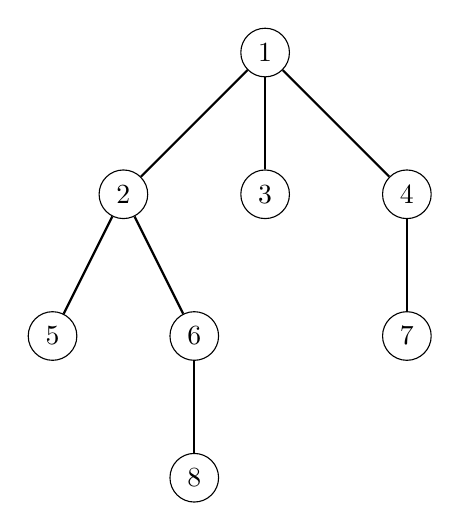
\begin{tikzpicture}[scale=0.9]
\node[draw, circle] (1) at (0,3) {$1$};
\node[draw, circle] (4) at (2,1) {$4$};
\node[draw, circle] (2) at (-2,1) {$2$};
\node[draw, circle] (3) at (0,1) {$3$};
\node[draw, circle] (7) at (2,-1) {$7$};
\node[draw, circle] (5) at (-3,-1) {$5$};
\node[draw, circle] (6) at (-1,-1) {$6$};
\node[draw, circle] (8) at (-1,-3) {$8$};
\path[draw,thick,-] (1) -- (2);
\path[draw,thick,-] (1) -- (3);
\path[draw,thick,-] (1) -- (4);
\path[draw,thick,-] (2) -- (5);
\path[draw,thick,-] (2) -- (6);
\path[draw,thick,-] (4) -- (7);
\path[draw,thick,-] (6) -- (8);
\end{tikzpicture}
\end{center}
\index{child}
\index{parent}

In a rooted tree, the \key{children} of a node
are its lower neighbors, and the \key{parent} of a node
is its upper neighbor.
Each node has exactly one parent,
except for the root that does not have a parent.
For example, in the above tree,
the children of node 2 are nodes 5 and 6,
and its parent is node 1.

\index{subtree}

The structure of a rooted tree is \emph{recursive}:
each node of the tree acts as the root of a \key{subtree}
that contains the node itself and all nodes
that are in the subtrees of its children.
For example, in the above tree, the subtree of node 2
consists of nodes 2, 5, 6 and 8:
\begin{center}
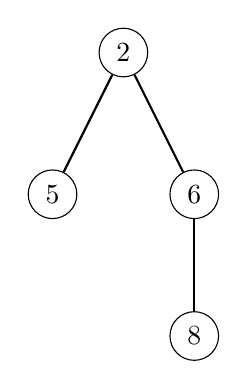
\begin{tikzpicture}[scale=0.9]
\node[draw, circle] (2) at (-2,1) {$2$};
\node[draw, circle] (5) at (-3,-1) {$5$};
\node[draw, circle] (6) at (-1,-1) {$6$};
\node[draw, circle] (8) at (-1,-3) {$8$};
\path[draw,thick,-] (2) -- (5);
\path[draw,thick,-] (2) -- (6);
\path[draw,thick,-] (6) -- (8);
\end{tikzpicture}
\end{center}

\section{Tree traversal}

General graph traversal algorithms
can be used to traverse the nodes of a tree.
However, the traversal of a tree is easier to implement than
that of a general graph, because
there are no cycles in the tree and it is not
possible to reach a node from multiple directions.

The typical way to traverse a tree is to start
a depth-first search at an arbitrary node.
The following recursive function can be used:

\begin{lstlisting}
void dfs(int s, int e) {
    // process node s
    for (auto u : adj[s]) {
        if (u != e) dfs(u, s);
    }
}
\end{lstlisting}

The function is given two parameters: the current node $s$
and the previous node $e$.
The purpose of the parameter $e$ is to make sure
that the search only moves to nodes
that have not been visited yet.

The following function call starts the search
at node $x$:

\begin{lstlisting}
dfs(x, 0);
\end{lstlisting}

In the first call $e=0$, because there is no
previous node, and it is allowed
to proceed to any direction in the tree.

\subsubsection{Dynamic programming}

Dynamic programming can be used to calculate
some information during a tree traversal.
Using dynamic programming, we can, for example,
calculate in $O(n)$ time for each node of a rooted tree the
number of nodes in its subtree
or the length of the longest path from the node
to a leaf.

As an example, let us calculate for each node $s$
a value $\texttt{count}[s]$: the number of nodes in its subtree.
The subtree contains the node itself and
all nodes in the subtrees of its children,
so we can calculate the number of nodes
recursively using the following code:

\begin{lstlisting}
void dfs(int s, int e) {
    count[s] = 1;
    for (auto u : adj[s]) {
        if (u == e) continue;
        dfs(u, s);
        count[s] += count[u];
    }
}
\end{lstlisting}

\section{Diameter}

\index{diameter}

The \key{diameter} of a tree
is the maximum length of a path between two nodes.
For example, consider the following tree:
\begin{center}
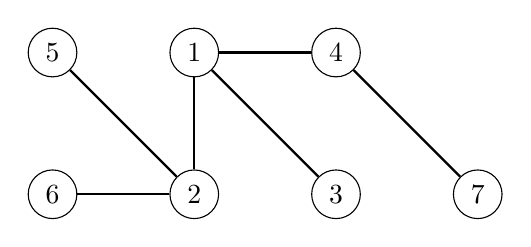
\begin{tikzpicture}[scale=0.9]
\node[draw, circle] (1) at (0,3) {$1$};
\node[draw, circle] (2) at (2,3) {$4$};
\node[draw, circle] (3) at (0,1) {$2$};
\node[draw, circle] (4) at (2,1) {$3$};
\node[draw, circle] (5) at (4,1) {$7$};
\node[draw, circle] (6) at (-2,3) {$5$};
\node[draw, circle] (7) at (-2,1) {$6$};
\path[draw,thick,-] (1) -- (2);
\path[draw,thick,-] (1) -- (3);
\path[draw,thick,-] (1) -- (4);
\path[draw,thick,-] (2) -- (5);
\path[draw,thick,-] (3) -- (6);
\path[draw,thick,-] (3) -- (7);
\end{tikzpicture}
\end{center}
The diameter of this tree is 4,
which corresponds to the following path:
\begin{center}
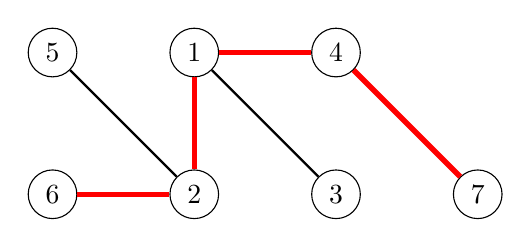
\begin{tikzpicture}[scale=0.9]
\node[draw, circle] (1) at (0,3) {$1$};
\node[draw, circle] (2) at (2,3) {$4$};
\node[draw, circle] (3) at (0,1) {$2$};
\node[draw, circle] (4) at (2,1) {$3$};
\node[draw, circle] (5) at (4,1) {$7$};
\node[draw, circle] (6) at (-2,3) {$5$};
\node[draw, circle] (7) at (-2,1) {$6$};
\path[draw,thick,-] (1) -- (2);
\path[draw,thick,-] (1) -- (3);
\path[draw,thick,-] (1) -- (4);
\path[draw,thick,-] (2) -- (5);
\path[draw,thick,-] (3) -- (6);
\path[draw,thick,-] (3) -- (7);

\path[draw,thick,-,color=red,line width=2pt] (7) -- (3);
\path[draw,thick,-,color=red,line width=2pt] (3) -- (1);
\path[draw,thick,-,color=red,line width=2pt] (1) -- (2);
\path[draw,thick,-,color=red,line width=2pt] (2) -- (5);
\end{tikzpicture}
\end{center}
Note that there may be several maximum-length paths.
In the above path, we could replace node 6 with node 5
to obtain another path with length 4.

Next we will discuss two $O(n)$ time algorithms
for calculating the diameter of a tree.
The first algorithm is based on dynamic programming,
and the second algorithm uses two depth-first searches.

\subsubsection{Algorithm 1}

A general way to approach many tree problems
is to first root the tree arbitrarily.
After this, we can try to solve the problem
separately for each subtree.
Our first algorithm for calculating the diameter
is based on this idea.

An important observation is that every path
in a rooted tree has a \emph{highest point}:
the highest node that belongs to the path.
Thus, we can calculate for each node the length
of the longest path whose highest point is the node.
One of those paths corresponds to the diameter of the tree.

For example, in the following tree,
node 1 is the highest point on the path
that corresponds to the diameter:
\begin{center}
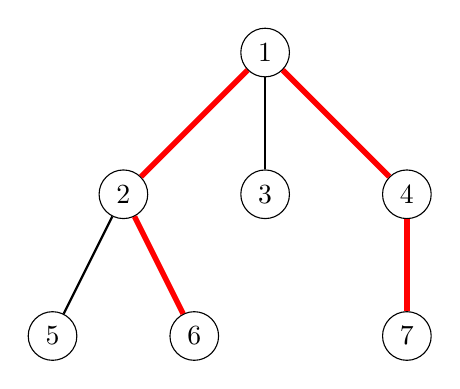
\begin{tikzpicture}[scale=0.9]
\node[draw, circle] (1) at (0,3) {$1$};
\node[draw, circle] (2) at (2,1) {$4$};
\node[draw, circle] (3) at (-2,1) {$2$};
\node[draw, circle] (4) at (0,1) {$3$};
\node[draw, circle] (5) at (2,-1) {$7$};
\node[draw, circle] (6) at (-3,-1) {$5$};
\node[draw, circle] (7) at (-1,-1) {$6$};
\path[draw,thick,-] (1) -- (2);
\path[draw,thick,-] (1) -- (3);
\path[draw,thick,-] (1) -- (4);
\path[draw,thick,-] (2) -- (5);
\path[draw,thick,-] (3) -- (6);
\path[draw,thick,-] (3) -- (7);

\path[draw,thick,-,color=red,line width=2pt] (7) -- (3);
\path[draw,thick,-,color=red,line width=2pt] (3) -- (1);
\path[draw,thick,-,color=red,line width=2pt] (1) -- (2);
\path[draw,thick,-,color=red,line width=2pt] (2) -- (5);
\end{tikzpicture}
\end{center}

We calculate for each node $x$ two values:
\begin{itemize}
\item $\texttt{toLeaf}(x)$: the maximum length of a path from $x$ to any leaf
\item $\texttt{maxLength}(x)$: the maximum length of a path
whose highest point is $x$
\end{itemize}
For example, in the above tree,
$\texttt{toLeaf}(1)=2$, because there is a path
$1 \rightarrow 2 \rightarrow 6$,
and $\texttt{maxLength}(1)=4$,
because there is a path
$6 \rightarrow 2 \rightarrow 1 \rightarrow 4 \rightarrow 7$.
In this case, $\texttt{maxLength}(1)$ equals the diameter.

Dynamic programming can be used to calculate the above
values for all nodes in $O(n)$ time.
First, to calculate $\texttt{toLeaf}(x)$,
we go through the children of $x$,
choose a child $c$ with maximum $\texttt{toLeaf}(c)$
and add one to this value.
Then, to calculate $\texttt{maxLength}(x)$,
we choose two distinct children $a$ and $b$
such that the sum $\texttt{toLeaf}(a)+\texttt{toLeaf}(b)$
is maximum and add two to this sum.

\subsubsection{Algorithm 2}

Another efficient way to calculate the diameter
of a tree is based on two depth-first searches.
First, we choose an arbitrary node $a$ in the tree
and find the farthest node $b$ from $a$.
Then, we find the farthest node $c$ from $b$.
The diameter of the tree is the distance between $b$ and $c$.

In the following graph, $a$, $b$ and $c$ could be:
\begin{center}
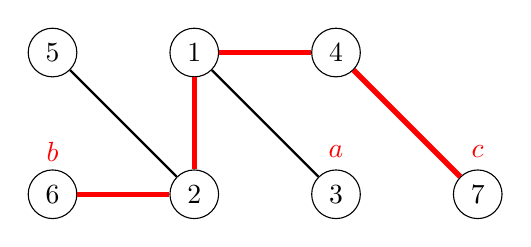
\begin{tikzpicture}[scale=0.9]
\node[draw, circle] (1) at (0,3) {$1$};
\node[draw, circle] (2) at (2,3) {$4$};
\node[draw, circle] (3) at (0,1) {$2$};
\node[draw, circle] (4) at (2,1) {$3$};
\node[draw, circle] (5) at (4,1) {$7$};
\node[draw, circle] (6) at (-2,3) {$5$};
\node[draw, circle] (7) at (-2,1) {$6$};
\path[draw,thick,-] (1) -- (2);
\path[draw,thick,-] (1) -- (3);
\path[draw,thick,-] (1) -- (4);
\path[draw,thick,-] (2) -- (5);
\path[draw,thick,-] (3) -- (6);
\path[draw,thick,-] (3) -- (7);
\node[color=red] at (2,1.6) {$a$};
\node[color=red] at (-2,1.6) {$b$};
\node[color=red] at (4,1.6) {$c$};

\path[draw,thick,-,color=red,line width=2pt] (7) -- (3);
\path[draw,thick,-,color=red,line width=2pt] (3) -- (1);
\path[draw,thick,-,color=red,line width=2pt] (1) -- (2);
\path[draw,thick,-,color=red,line width=2pt] (2) -- (5);
\end{tikzpicture}
\end{center}

This is an elegant method, but why does it work?

It helps to draw the tree differently so that
the path that corresponds to the diameter
is horizontal, and all other
nodes hang from it:
\begin{center}
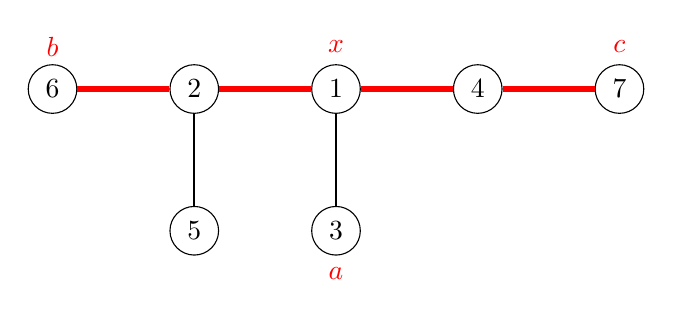
\begin{tikzpicture}[scale=0.9]
\node[draw, circle] (1) at (2,1) {$1$};
\node[draw, circle] (2) at (4,1) {$4$};
\node[draw, circle] (3) at (0,1) {$2$};
\node[draw, circle] (4) at (2,-1) {$3$};
\node[draw, circle] (5) at (6,1) {$7$};
\node[draw, circle] (6) at (0,-1) {$5$};
\node[draw, circle] (7) at (-2,1) {$6$};
\path[draw,thick,-] (1) -- (2);
\path[draw,thick,-] (1) -- (3);
\path[draw,thick,-] (1) -- (4);
\path[draw,thick,-] (2) -- (5);
\path[draw,thick,-] (3) -- (6);
\path[draw,thick,-] (3) -- (7);
\node[color=red] at (2,-1.6) {$a$};
\node[color=red] at (-2,1.6) {$b$};
\node[color=red] at (6,1.6) {$c$};
\node[color=red] at (2,1.6) {$x$};

\path[draw,thick,-,color=red,line width=2pt] (7) -- (3);
\path[draw,thick,-,color=red,line width=2pt] (3) -- (1);
\path[draw,thick,-,color=red,line width=2pt] (1) -- (2);
\path[draw,thick,-,color=red,line width=2pt] (2) -- (5);
\end{tikzpicture}
\end{center}

Node $x$ indicates the place where the path
from node $a$ joins the path that corresponds
to the diameter.
The farthest node from $a$
is node $b$, node $c$ or some other node
that is at least as far from node $x$.
Thus, this node is always a valid choice for
an endpoint of a path that corresponds to the diameter.

\section{All longest paths}

Our next problem is to calculate for every node
in the tree the maximum length of a path
that begins at the node.
This can be seen as a generalization of the
tree diameter problem, because the largest of those
lengths equals the diameter of the tree.
Also this problem can be solved in $O(n)$ time.

As an example, consider the following tree:
\begin{center}
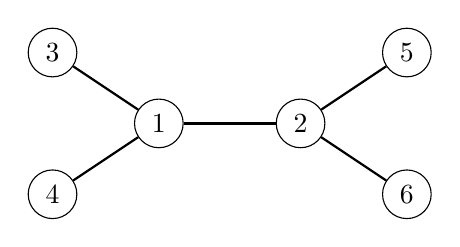
\begin{tikzpicture}[scale=0.9]
\node[draw, circle] (1) at (0,0) {$1$};
\node[draw, circle] (2) at (-1.5,-1) {$4$};
\node[draw, circle] (3) at (2,0) {$2$};
\node[draw, circle] (4) at (-1.5,1) {$3$};
\node[draw, circle] (6) at (3.5,-1) {$6$};
\node[draw, circle] (7) at (3.5,1) {$5$};
\path[draw,thick,-] (1) -- (2);
\path[draw,thick,-] (1) -- (3);
\path[draw,thick,-] (1) -- (4);
\path[draw,thick,-] (3) -- (6);
\path[draw,thick,-] (3) -- (7);
\end{tikzpicture}
\end{center}

Let $\texttt{maxLength}(x)$ denote the maximum length
of a path that begins at node $x$.
For example, in the above tree,
$\texttt{maxLength}(4)=3$, because there
is a path $4 \rightarrow 1 \rightarrow 2 \rightarrow 6$.
Here is a complete table of the values:
\begin{center}
\begin{tabular}{l|lllllll}
node $x$ & 1 & 2 & 3 & 4 & 5 & 6 \\
$\texttt{maxLength}(x)$ & 2 & 2 & 3 & 3 & 3 & 3 \\
\end{tabular}
\end{center}

Also in this problem, a good starting point
for solving the problem is to root the tree arbitrarily:
\begin{center}
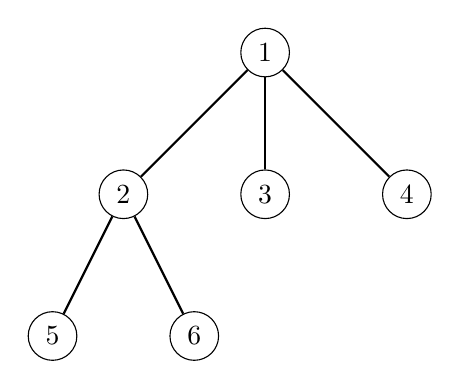
\begin{tikzpicture}[scale=0.9]
\node[draw, circle] (1) at (0,3) {$1$};
\node[draw, circle] (2) at (2,1) {$4$};
\node[draw, circle] (3) at (-2,1) {$2$};
\node[draw, circle] (4) at (0,1) {$3$};
\node[draw, circle] (6) at (-3,-1) {$5$};
\node[draw, circle] (7) at (-1,-1) {$6$};
\path[draw,thick,-] (1) -- (2);
\path[draw,thick,-] (1) -- (3);
\path[draw,thick,-] (1) -- (4);
\path[draw,thick,-] (3) -- (6);
\path[draw,thick,-] (3) -- (7);
\end{tikzpicture}
\end{center}

The first part of the problem is to calculate for every node $x$
the maximum length of a path that goes through a child of $x$.
For example, the longest path from node 1
goes through its child 2:
\begin{center}
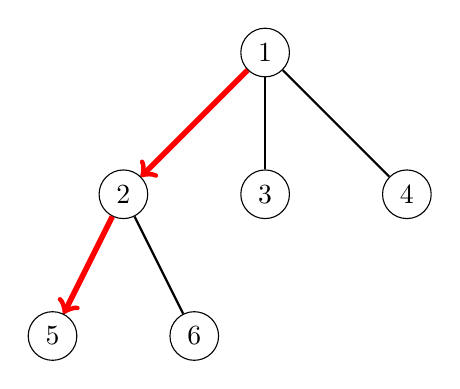
\begin{tikzpicture}[scale=0.9]
\node[draw, circle] (1) at (0,3) {$1$};
\node[draw, circle] (2) at (2,1) {$4$};
\node[draw, circle] (3) at (-2,1) {$2$};
\node[draw, circle] (4) at (0,1) {$3$};
\node[draw, circle] (6) at (-3,-1) {$5$};
\node[draw, circle] (7) at (-1,-1) {$6$};
\path[draw,thick,-] (1) -- (2);
\path[draw,thick,-] (1) -- (3);
\path[draw,thick,-] (1) -- (4);
\path[draw,thick,-] (3) -- (6);
\path[draw,thick,-] (3) -- (7);

\path[draw,thick,->,color=red,line width=2pt] (1) -- (3);
\path[draw,thick,->,color=red,line width=2pt] (3) -- (6);
\end{tikzpicture}
\end{center}
This part is easy to solve in $O(n)$ time, because we can use
dynamic programming as we have done previously.

Then, the second part of the problem is to calculate
for every node $x$ the maximum length of a path
through its parent $p$.
For example, the longest path
from node 3 goes through its parent 1:
\begin{center}
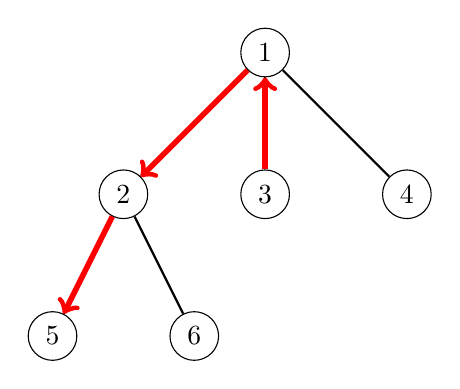
\begin{tikzpicture}[scale=0.9]
\node[draw, circle] (1) at (0,3) {$1$};
\node[draw, circle] (2) at (2,1) {$4$};
\node[draw, circle] (3) at (-2,1) {$2$};
\node[draw, circle] (4) at (0,1) {$3$};
\node[draw, circle] (6) at (-3,-1) {$5$};
\node[draw, circle] (7) at (-1,-1) {$6$};
\path[draw,thick,-] (1) -- (2);
\path[draw,thick,-] (1) -- (3);
\path[draw,thick,-] (1) -- (4);
\path[draw,thick,-] (3) -- (6);
\path[draw,thick,-] (3) -- (7);

\path[draw,thick,->,color=red,line width=2pt] (4) -- (1);
\path[draw,thick,->,color=red,line width=2pt] (1) -- (3);
\path[draw,thick,->,color=red,line width=2pt] (3) -- (6);
\end{tikzpicture}
\end{center}

At first glance, it seems that we should choose
the longest path from $p$.
However, this \emph{does not} always work,
because the longest path from $p$
may go through $x$.
Here is an example of this situation:
\begin{center}
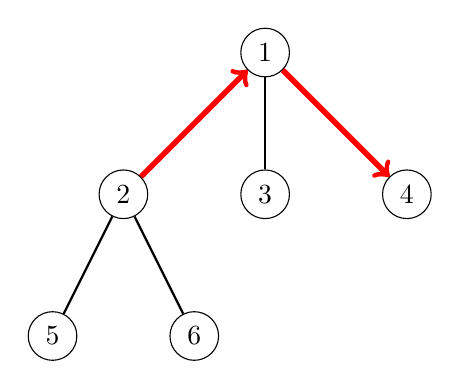
\begin{tikzpicture}[scale=0.9]
\node[draw, circle] (1) at (0,3) {$1$};
\node[draw, circle] (2) at (2,1) {$4$};
\node[draw, circle] (3) at (-2,1) {$2$};
\node[draw, circle] (4) at (0,1) {$3$};
\node[draw, circle] (6) at (-3,-1) {$5$};
\node[draw, circle] (7) at (-1,-1) {$6$};
\path[draw,thick,-] (1) -- (2);
\path[draw,thick,-] (1) -- (3);
\path[draw,thick,-] (1) -- (4);
\path[draw,thick,-] (3) -- (6);
\path[draw,thick,-] (3) -- (7);

\path[draw,thick,->,color=red,line width=2pt] (3) -- (1);
\path[draw,thick,->,color=red,line width=2pt] (1) -- (2);
\end{tikzpicture}
\end{center}

Still, we can solve the second part in
$O(n)$ time by storing \emph{two} maximum lengths
for each node $x$:
\begin{itemize}
\item $\texttt{maxLength}_1(x)$:
the maximum length of a path from $x$
\item $\texttt{maxLength}_2(x)$
the maximum length of a path from $x$
in another direction than the first path
\end{itemize}
For example, in the above graph,
$\texttt{maxLength}_1(1)=2$
using the path $1 \rightarrow 2 \rightarrow 5$,
and $\texttt{maxLength}_2(1)=1$
using the path $1 \rightarrow 3$.

Finally, if the path that corresponds to
$\texttt{maxLength}_1(p)$ goes through $x$,
we conclude that the maximum length is
$\texttt{maxLength}_2(p)+1$,
and otherwise the maximum length is
$\texttt{maxLength}_1(p)+1$.


\section{Binary trees}

\index{binary tree}

\begin{samepage}
A \key{binary tree} is a rooted tree
where each node has a left and right subtree.
It is possible that a subtree of a node is empty.
Thus, every node in a binary tree has
zero, one or two children.

For example, the following tree is a binary tree:
\begin{center}
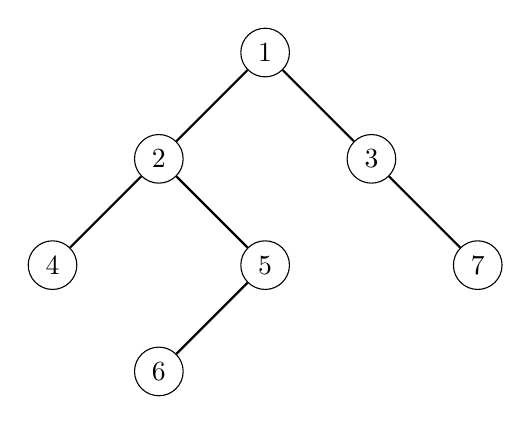
\begin{tikzpicture}[scale=0.9]
\node[draw, circle] (1) at (0,0) {$1$};
\node[draw, circle] (2) at (-1.5,-1.5) {$2$};
\node[draw, circle] (3) at (1.5,-1.5) {$3$};
\node[draw, circle] (4) at (-3,-3) {$4$};
\node[draw, circle] (5) at (0,-3) {$5$};
\node[draw, circle] (6) at (-1.5,-4.5) {$6$};
\node[draw, circle] (7) at (3,-3) {$7$};

\path[draw,thick,-] (1) -- (2);
\path[draw,thick,-] (1) -- (3);
\path[draw,thick,-] (2) -- (4);
\path[draw,thick,-] (2) -- (5);
\path[draw,thick,-] (5) -- (6);
\path[draw,thick,-] (3) -- (7);
\end{tikzpicture}
\end{center}
\end{samepage}

\index{pre-order}
\index{in-order}
\index{post-order}

The nodes of a binary tree have three natural
orderings that correspond to different ways to 
recursively traverse the tree:

\begin{itemize}
\item \key{pre-order}: first process the root,
then traverse the left subtree, then traverse the right subtree
\item \key{in-order}: first traverse the left subtree,
then process the root, then traverse the right subtree
\item \key{post-order}: first traverse the left subtree,
then traverse the right subtree, then process the root
\end{itemize}

For the above tree, the nodes in
pre-order are
$[1,2,4,5,6,3,7]$,
in in-order $[4,2,6,5,1,3,7]$
and in post-order $[4,6,5,2,7,3,1]$.

If we know the pre-order and in-order
of a tree, we can reconstruct the exact structure of the tree.
For example, the above tree is the only possible tree
with pre-order $[1,2,4,5,6,3,7]$ and
in-order $[4,2,6,5,1,3,7]$.
In a similar way, the post-order and in-order
also determine the structure of a tree.

However, the situation is different if we only know
the pre-order and post-order of a tree.
In this case, there may be more than one tree
that match the orderings.
For example, in both of the trees
\begin{center}
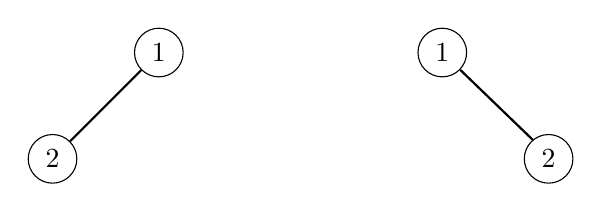
\begin{tikzpicture}[scale=0.9]
\node[draw, circle] (1) at (0,0) {$1$};
\node[draw, circle] (2) at (-1.5,-1.5) {$2$};
\path[draw,thick,-] (1) -- (2);

\node[draw, circle] (1b) at (0+4,0) {$1$};
\node[draw, circle] (2b) at (1.5+4,-1.5) {$2$};
\path[draw,thick,-] (1b) -- (2b);
\end{tikzpicture}
\end{center}
the pre-order is $[1,2]$ and the post-order is $[2,1]$,
but the structures of the trees are different.

